\documentclass[a4paper]{article}

\usepackage[english]{babel}
\usepackage[utf8]{inputenc}
\usepackage{amsmath}
\usepackage{graphicx}
\usepackage[colorinlistoftodos]{todonotes}

\title{Behaviour Dynamics in Social Networks - Assignment 1}

\author{Maria Hotoiu, Federico Tavella}

\date{\today}

\begin{document}
\maketitle

\begin{abstract}
After Jenny has entered Mark’s door, her presence clearly makes that Mark becomes happy. Liking Mark a lot, his happiness makes her nervous, which makes that she breaks one of the two nice vases near the door. Seeing this, Mark becomes angry on her. This makes Jenny sad. Jenny’s sadness makes Mark’s anger disappear, and he gives Jenny a hug. Seeing this, Mark’s partner Dion becomes jealous, upon which she breaks the other vase.
\newline
Use the concepts and formats introduced in Chapter 2 to analyse and model this scenario by a temporal-causal network by the following steps.
\end{abstract}

\section{Graphical conceptual representation}
\label{sec:graphical_conceptual_representation}

States describing the scenario:

\begin{enumerate}
\item Jenny's presence ($X_1$);
\item Mark becomes happy ($X_2$);
\item Jenny likes Mark ($X_3$);
\item Jenny becomes nervous ($X_4$);
\item Jenny breaks a vase ($X_5$);
\item Mark becomes angry ($X_6$);
\item Jenny becomes sad ($X_7$);
\item Mark gives Jenny a hug ($X_8$);
\item Dion become jealous ($X_9$);
\item Dion breaks a vase ($X_10$).
\end{enumerate}

In Figure~\ref{fig:graphical_conceptual_representation}, we can observe a connection that models a negative impact in order to make the level of the affected state lower - the one going from $X_7$ to $X_6$ (i.e. Mark anger decreases due to Jenny sadness). There is also a loop that contains two states: $X_6$ and $X_7$.


\begin{figure}[!htbp]
\center
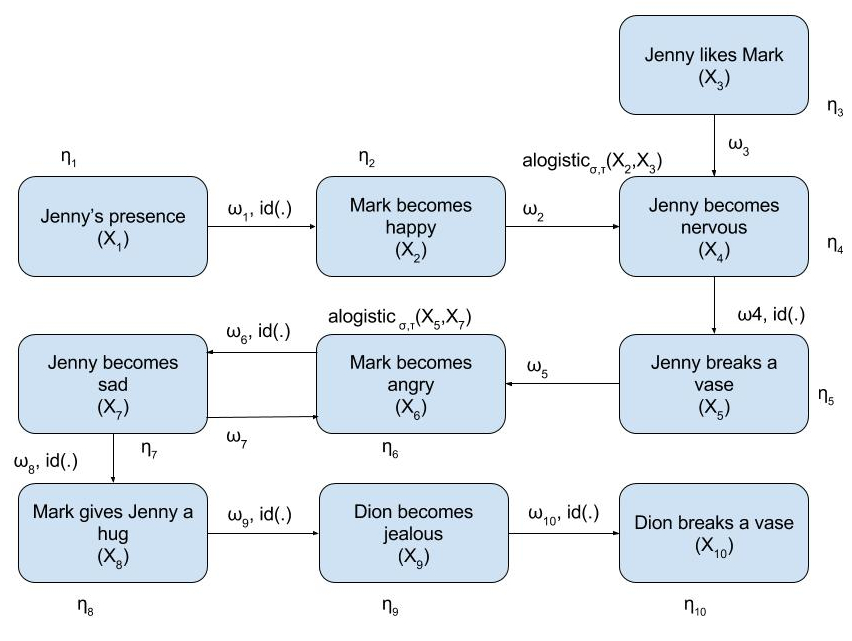
\includegraphics[width=\textwidth]{res/img/graphical_conceptual_representation}
\caption{Conceptual representation of the scenario.}
\label{fig:graphical_conceptual_representation}
\end{figure}

\section{Conceptual representation in matrix format}

We now move to the matrix representation of the graph in Figure~\ref{fig:graphical_conceptual_representation}. Rows represent nodes from which edges are starting, while columns represent nodes in which edges are ending.

\begin{figure}[!htbp]
\centering
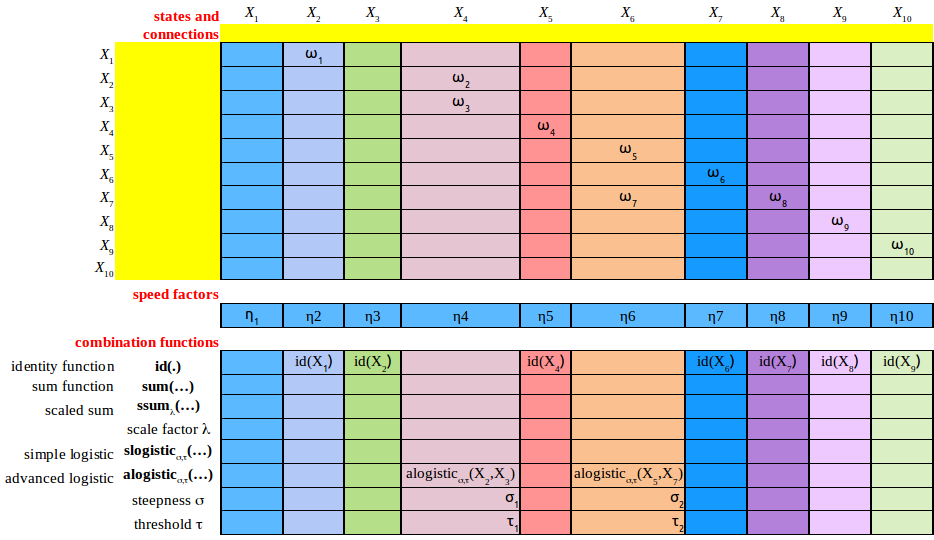
\includegraphics[width=\textwidth]{res/img/matrix_conceptual_representation}
\caption{Matrix format of the conceptual representation}
\label{fig:matrix_conceptual_representation}
\end{figure}

\section{Numerical representation}

Numerical representation for the scenario represented in Figure \ref{fig:matrix_conceptual_representation}.

\subsection{Difference equation}

Initial states:
\begin{equation}
X_{1}(t+\Delta t) = X_{1}(t) + \eta_{1} ( id(X_{1}(t)) - X_{1}(t))\Delta t = X_{1}(t)
\end{equation}
\begin{equation}
X_{3}(t+\Delta t) = X_{3}(t) + \eta_{3} ( id(X_{3}(t)) - X_{3}(t))\Delta t = X_{3}(t)
\end{equation}
\\
Intermediate states:
\begin{equation}
X_{2}(t+\Delta t) = X_{2}(t) + \eta_{2} (id(\omega_{2} X_{1}(t)) - X_{2}(t))\Delta t
\end{equation}
\begin{equation}
X_{4}(t+\Delta t) = X_{4}(t) + \eta_{4} ( alogistic_{\sigma ,\tau}(\omega_{2} X_{2}(t),\omega_{3} X_{3}(t)) - X_{4}(t))\Delta t
\end{equation}
\begin{equation}
X_{5}(t+\Delta t) = X_{5}(t) + \eta_{5} (id(\omega_{4} X_{4}(t)) - X_{5}(t))\Delta t
\end{equation}
\begin{equation}
X_{6}(t+\Delta t) = X_{6}(t) + \eta_{6} (alogistic_{\sigma ,\tau}(\omega_{5} X_{5}(t),\omega_{7} X_{7}(t)) - X_{6}(t))\Delta t
\end{equation}
\begin{equation}
X_{7}(t+\Delta t) = X_{7}(t) + \eta_{7} (id(\omega_{6} X_{6}(t)) - X_{7}(t))\Delta t
\end{equation}
\begin{equation}
X_{8}(t+\Delta t) = X_{8}(t) + \eta_{8} (id(\omega_{8} X_{7}(t)) - X_{8}(t))\Delta t
\end{equation}
\begin{equation}
X_{9}(t+\Delta t) = X_{9}(t) + \eta_{9} (id(\omega_{9} X_{8}(t)) - X_{9}(t))\Delta t
\end{equation}
\\
Final state:
\begin{equation}
X_{10}(t+\Delta t) = X_{10}(t) + \eta_{10} (id(\omega_{10} X_{9}(t)) - X_{10}(t))\Delta t
\end{equation}


\subsection{Differential equation}

\begin{equation}
\frac{\delta X_{1}(t)}{\delta t} = X_{1}(t) + \eta_{1} \cdot ( id(X_{1}(t)) - X_{1}(t))
\end{equation}

\section{Expected behaviour}






\section{Simulation}

\begin{figure}[!htbp]
\center
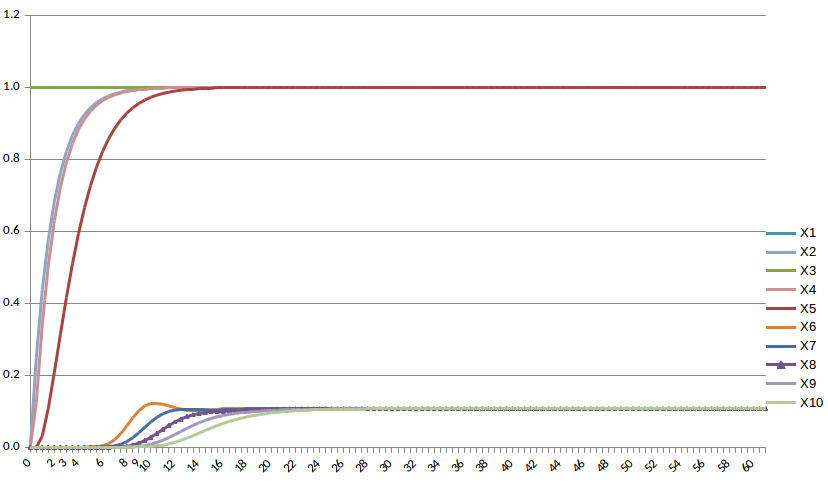
\includegraphics[width=\textwidth]{res/img/numerical_representation}
\end{figure}



%\begin{thebibliography}{9}
%\bibitem{nano3}
%  K. Grove-Rasmussen og Jesper Nygård,
%  \emph{Kvantefænomener i Nanosystemer}.
%  Niels Bohr Institute \& Nano-Science Center, Københavns Universitet

%\end{thebibliography}
\end{document}
